\documentclass[class=jsarticle, crop=false, dvipdfmx, fleqn]{standalone}
\input{/Users/User/Documents/University/report_template/preamble/preamble}
\begin{document}

\section*{宿題1}

\subsection*{(1)}

拡張特徴ベクトル・拡張重みベクトル・正規化を実装し,
パーセプトロン (バッチもしくはオンライン) を実装する。
また,
Linearly separable (linear)・Linearly non-separable (nonlinear)・Skewed linearly separable (slinear)の3種類のデータについてパーセプトロンを実行し,
その振る舞いを調べる。
なお,括弧書きで略称を示した。
以降は略称を用いる。

拡張重みの更新式は次のようになる。
\begin{eqnarray}
    w^{(t+1)} = w^{(t)} + \rho \sum_{x \in \tilde{X}} x
\end{eqnarray}
ここで,\(t\)は更新回数,
\(\rho\)は学習率,
\(\tilde{X}\)は識別誤りとなっているすべてのサンプルである。
これを実装すればよい。

データは全て2カテゴリからなる二次元点群で,
slinearのみ500サンプル,
他の2つは100サンプルある。
本来,学習の終了条件は点が全て正しいカテゴリに分類されたときであるが,
この設定では収束しない場合があるので。
更新を100回行ったときも学習を終了させる。
学習率\(\rho = 0.1\)としたときの結果を以下の表\ref{tab:result1}に,
各データの点群と境界のプロットを図\ref{fig:result1_linear}--\ref{fig:result1_slinear}に示す。

結果から,線形分離可能なデータ(linear)や,
完全に線形分離するのは不可能だが大半がうまく分けられるようなデータ(slinear)
に対しては,
パーセプトロンはうまく機能することがわかる。
一方,線形分離不可能なデータ(nonlinear)に対しては当然全く機能しない。
また,学習中の境界の挙動を観察した結果を以下に記す。
linearについては,図\ref{fig:result1_linear}にある最終的に得られる境界を中心に,
それとほぼ平行に減衰振動するような形で境界が移動していき,
最終的に収束した。
nonlinearについては,
境界がプロットの範囲中に現れては消えることを繰り返し続け,
最後まで振動し続けていた。
slinearについては,
まず図\ref{fig:result1_slinear}の右上と左上を線対称に置くような位置に境界が引かれ,
そこから徐々に立ち上がっていき,
最終的に図の中心付近の点を(ある程度)うまく分類できるようになった。
linearを減衰振動,nonlinearを振動と表現したことに倣うと,
slinearは過減衰のような挙動であった。


\begin{table}
    \centering
    \caption{結果}
    \begin{tabular}{lcccrr}
        データの種類 & \(w_0\) & \(w_1\) & \(w_2\) & 識別誤り数 & 識別誤り率 \\ \hline
        linear & \(-1.002\) & 4.727 & 2.401 & 0 & 0{\%} \\
        nonlinear & \(-4.002\) & 1.870 & \(-0.1073\) & 38 & 38{\%} \\
        slinear & \(-0.2024\) & 20.30 & 0.01964 & 2 & 0.4{\%}
    \end{tabular}
    \label{tab:result1}
\end{table}

\begin{figure}
    \centering
    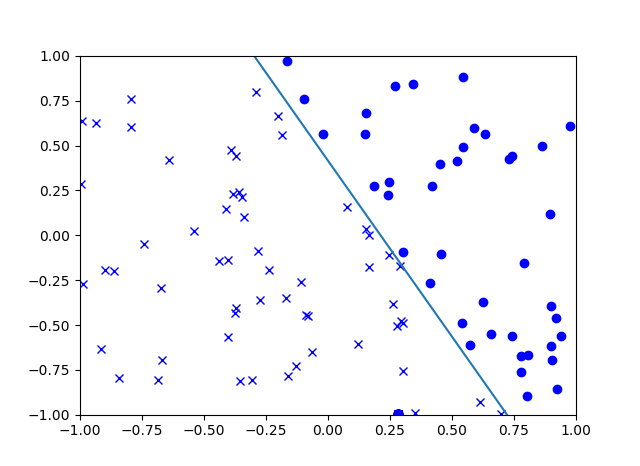
\includegraphics[clip, width=12cm]{../figures/assignment1_1_linear_result}
    \caption{linearデータに対してパーセプトロンを適用したときの点群と境界}
    \label{fig:result1_linear}
\end{figure}

\begin{figure}
    \centering
    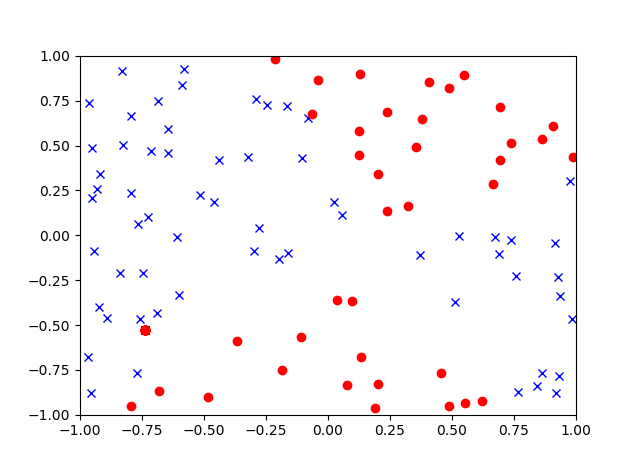
\includegraphics[clip, width=12cm]{../figures/assignment1_1_nonlinear_result}
    \caption{nonlinearデータに対してパーセプトロンを適用したときの点群と境界}
    \label{fig:result1_nonlinear}
\end{figure}

\begin{figure}
    \centering
    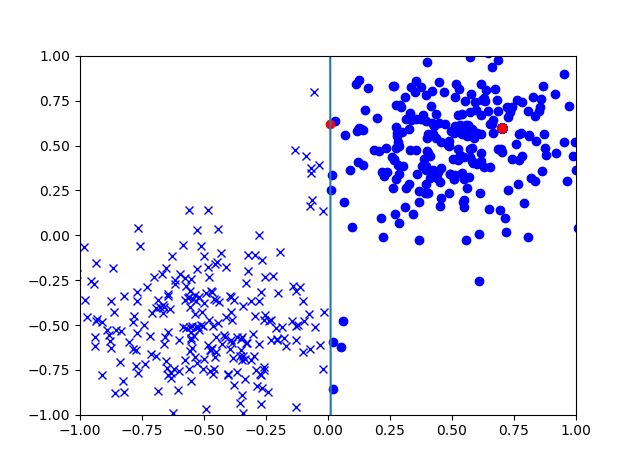
\includegraphics[clip, width=12cm]{../figures/assignment1_1_slinear_result}
    \caption{slinearデータに対してパーセプトロンを適用したときの点群と境界}
    \label{fig:result1_slinear}
\end{figure}



\clearpage
\subsection*{(2)}

MSE法による識別器を実装し,3種類のデータにより学習させる。
また,その振る舞いについて調べる。

重みの解析解は次のようになる。
\begin{equation}
    \bm{w} = (\bm{X}^\mathrm{T} \bm{X})^{-1} X^\mathrm{T} \bm{y}
\end{equation}
また,LMS法を用いるときの,拡張重みの更新式は次のようになる。
\begin{equation}
    \hat{\bm{w}}^{(t+1)} = \hat{\bm{w}}^{(t)} - \rho \qty(\hat{\bm{w}}^\mathrm{T} \hat{\bm{x}} - \bm{y}) \hat{\bm{x}}
\end{equation}

学習の終了条件は重みの変化量のノルムが\num{1e-5}以下となったときとする。
今回は学習率をデータごとに変えたため,それも結果にまとめて記すこととする。
結果を以下の表\ref{tab:result2}に,
各データの点群と境界のプロットを図\ref{fig:result2_linear}--\ref{fig:result2_slinear}に示す。

結果はパーセプトロンのときと同様,linearとslinearに対してはある程度対応でき,
nonlinearに対してはうまくいかないというものになった。
また,精度はパーセプトロンよりも劣る形となった。
しかし,パーセプトロンと異なり,
学習の終了条件が実現可能なものになっており,
更新回数で切り上げないと収束せず無限ループに陥るということが起きないのは利点である。
また,学習中の境界の挙動は,
勾配降下法を用いているため,
当然減衰振動のようなものとなった。



\begin{table}
    \centering
    \caption{結果}
    \begin{tabular}{lccccrr}
        データの種類 & 学習率 & \(w_0\) & \(w_1\) & \(w_2\) & 識別誤り数 & 識別誤り率 \\ \hline
        linear & 0.015 & \(-0.2164\) & 1.379 & 0.6243 & 6 & 6{\%} \\
        nonlinear & 0.015 & \(-0.2141\) & 0.5494 & 0.03766 & 39 & 39{\%} \\
        slinear & 0.001 & \(-0.007554\) & 1.035 & 0.7157 & 13 & 2.6{\%}
    \end{tabular}
    \label{tab:result2}
\end{table}

\begin{figure}
    \centering
    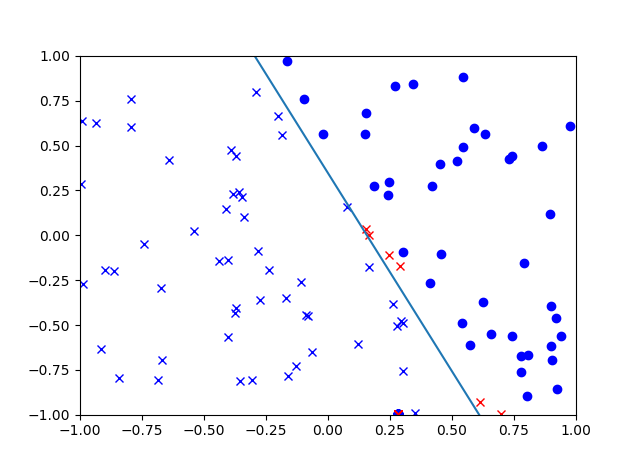
\includegraphics[clip, width=12cm]{../figures/assignment1_2_linear_result}
    \caption{linearデータに対してMSE法を適用したときの点群と境界}
    \label{fig:result2_linear}
\end{figure}

\begin{figure}
    \centering
    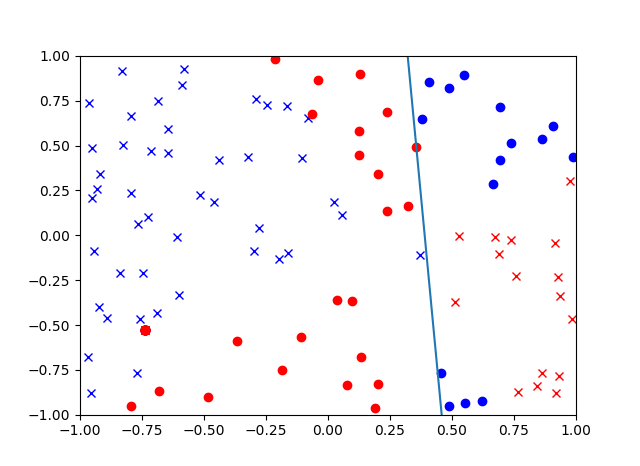
\includegraphics[clip, width=12cm]{../figures/assignment1_2_nonlinear_result}
    \caption{nonlinearデータに対してMSE法を適用したときの点群と境界}
    \label{fig:result2_nonlinear}
\end{figure}

\begin{figure}
    \centering
    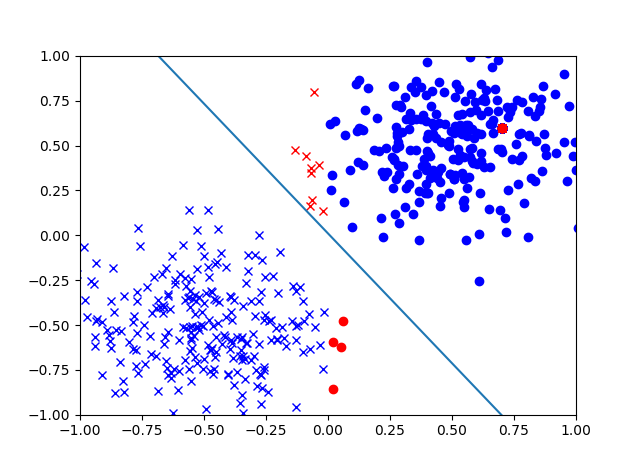
\includegraphics[clip, width=12cm]{../figures/assignment1_2_slinear_result}
    \caption{slinearデータに対してMSE法を適用したときの点群と境界}
    \label{fig:result2_slinear}
\end{figure}


\end{document}
